\title{
\centering

\includegraphics[width=4cm,height=4cm,keepaspectratio]{du.jpg} \\ \ CSE - 4255 Data Mining and Warehousing Lab\\  \Large \textit{Comparison Between the Performance of Apriori and FP-growth Algorithm in Frequent Pattern Mining}\\}


\author{
        Saif Mahmud \\
        Roll: SH - 54\\
            \and
        M. Tanjid Hasan Tonmoy\\
        Roll: SH - 09\\
            \and
        \\\textbf{Submitted To:}\\ Dr. Chowdhury Farhan Ahmed \\
        Professor\\
        \\ \& \\ 
        Abu Ahmed Ferdaus\\
        Associate Professor\\ \\
        Department of Computer Science and Engineering\\
        University of Dhaka        
}
\date{\today}

\documentclass[12pt]{article}
\usepackage{graphicx}
\usepackage{cite}
\usepackage{url}
\usepackage{multirow}
%\usepackage[a4paper]{geometry}
\newcommand{\s}{\vspace{0.2cm}}
\usepackage{float}

\begin{document}


\maketitle
\thispagestyle{empty}
\clearpage
\newpage

\section{Problem Definition}
In this experiment, we have implemented prefix trie based apriori algorithm and FP-growth algorithm to mine frequent patterns in transactional database. The performance in terms of execution time is compared through setting same minimum support threshold for six different datasets.


\section{Theory}

\subsection{Apriori Algorithm}
Apriori employs an iterative approach known as a level-wise search, where k-itemsets are used to explore (k + 1)-itemsets. To improve the efficiency of the level-wise generation of frequent itemsets, an important property called the Apriori property is used to reduce the search space. This property is described as all the nonempty subsets of a frequent itemset must also be frequent. Steps required for finding frequent patterns of level i are given below:
\begin{itemize}
	\item To find $L_k$, a set of candidate k-itemsets is generated by joining $L_{k-1}$ with itself.
	\item To reduce the size of $C_k$, the Apriori property is used as follows. Any (k − 1)-itemset that is not frequent cannot be a subset of a frequent k-itemset. Hence, if any (k - 1)-subset of a candidate k-itemset is not in $ L_{k-1} $, then the candidate cannot be frequent either and so can be removed from $ C_k $.
	\item The support count of candidates at any particular level has been computed through constructing a prefix trie based on the itemsets in $ C_k $ and single database scan to assign a frequency to the nodes. 
	
\end{itemize}

\subsection{FP-Growth Algorithm}
Frequent Pattern growth or simply FP-growth adopts a divide-and-conquer strategy as follows :
\subsubsection{FP-tree construction}
\begin{itemize}
	\item Scan database once and find support frequencies for each item.
	\item Discard infrequent items and sort frequent items in decreasing order based on their support. The frequent 1-items are stored in a header table.
	\item With a databse scan, the transactions are inserted in a prefix trie. Items in each transaction are sorted by the sequence in the header table and items containing support count less than the minimum support count are discarded from the transaction. Header table contains information which item is contained in which nodes in the FP-Tree through node links.
	
\end{itemize}

\subsubsection{Frequent Pattern Extraction}
\begin{itemize}
	\item FP-Growth extracts frequent itemsets from the FP-tree in a bottom-up algorithm from the leaves towards the root.
	\item Construct a conditional pattern base from the FP-Tree and conditional FP-Tree from the conditional pattern base.
	\item Perform mining recursively on the FP-tree to generate all the frequent patterns. The pattern generation is done by concatenation of suffix pattern with frequent patterns generated from the FP-Tree recursively.
	
\end{itemize}

\section{Experimental Setup}
\subsection{Implementation}

For the implementation of the apriori algorithm, a trie data structure has been utilized at each level. The candidates are used to build the data structure and the database is scanned to obtain the support count for all candidates. 

For FP-growth, FP-tree data structure has been used. The tree is built recursively once and is used to build FP-tree at further steps.

\subsection{Datasets}
For the experiments, five datasets and at least five minimum support threshold for each dataset have been used which has been summarized in Table 1.


\begin{table}[]
	\label{tab:data}
	\caption{Dataset Statistics}
	\begin{tabular}{|c|c|c|c|}
		\hline
		\textbf{Dataset} & \textbf{\begin{tabular}[c]{@{}c@{}}Average \\ Transaction Length\end{tabular}} & \textbf{\begin{tabular}[c]{@{}c@{}}No of \\ Transactions\end{tabular}} & \textbf{Threshold (Percentage)} \\ \hline
		Mushroom         & 23                                                                             & 8124                                                                   & 20 - 40                         \\ \hline
		Chess            & 37                                                                             & 3196                                                                   & 75 - 95                         \\ \hline
		Retail           & 10.30576                                                                       & 88162                                                                  & 0.5 - 15                        \\ \hline
		Pumsb            & 74.0                                                                           & 49046                                                                  & 90 - 98                         \\ \hline
		Pumsb\_star      & 50.48214                                                                       & 49046                                                                  & 40 - 65                         \\ \hline
		Kosarak          & 8.099999                                                                       & 990002                                                                 & 0.5 - 15                        \\ \hline
	\end{tabular}
\end{table}


\section{Result}
The obtained results are presented in the figures where the x-axis represents the minimum support threshold and the y-axis represents the execution time. It is evident that in case of lower minimum support threshold there is acute difference in the execution time which is diminished as the minimum support increases.

\begin{figure}[H]
	\centering
	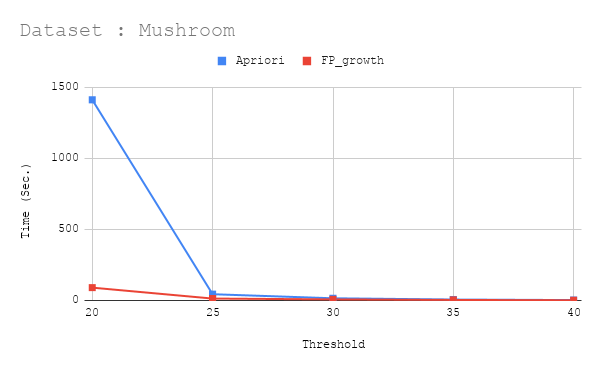
\includegraphics[width = 0.95\columnwidth, height = 7.5cm]{Mushroom.png}
	\caption{Dataset - Mushroom}
	\label{fig:mushroom}
\end{figure}

\begin{figure}[H]
	\centering
	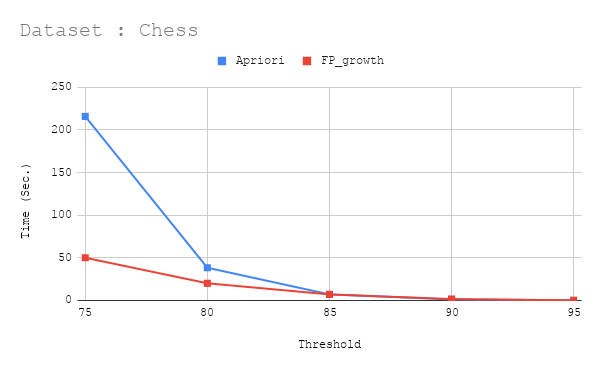
\includegraphics[width = 0.95\columnwidth, height = 7.5cm]{Chess.png}
	\caption{Dataset - Chess}
	\label{fig:chess}
\end{figure}

\begin{figure}[H]
	\centering
	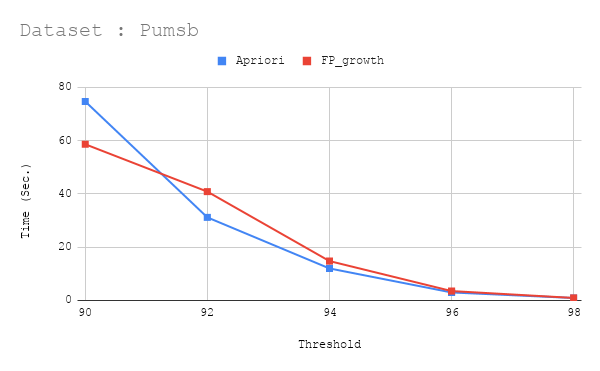
\includegraphics[width = 0.95\columnwidth, height = 7.5cm]{Pumsb.png}
	\caption{Dataset - Pumsb}
	\label{fig:pumsb}
\end{figure}

\begin{figure}[H]
	\centering
	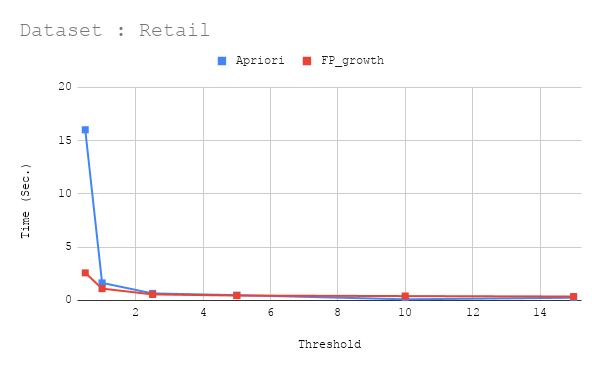
\includegraphics[width = 0.95\columnwidth, height = 7.5cm]{Retail.png}
	\caption{Dataset - Retail}
	\label{fig:retail}
\end{figure}

\begin{figure}[H]
	\centering
	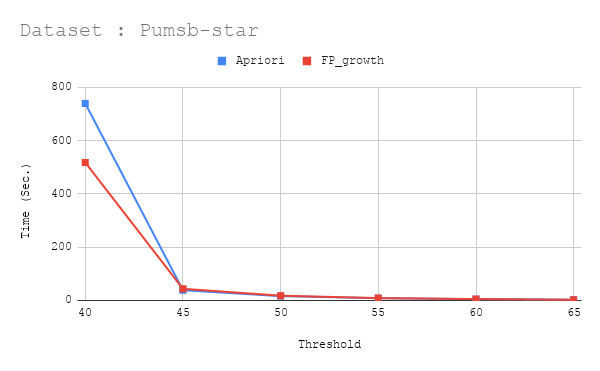
\includegraphics[width = 0.95\columnwidth, height = 7.5cm]{Pumsb-star.png}
	\caption{Dataset - Pumsb Star}
	\label{fig:pbs}
\end{figure}

\begin{figure}[H]
	\centering
	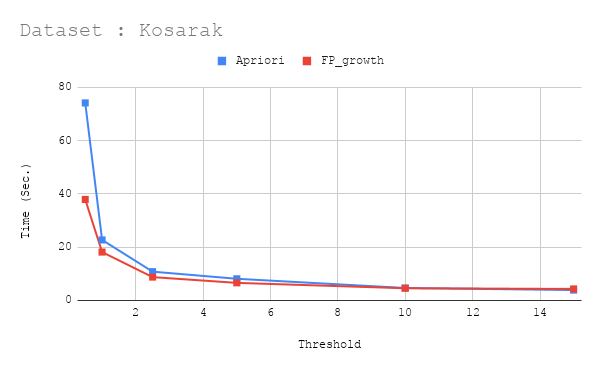
\includegraphics[width = 0.95\columnwidth, height = 8.5cm]{Kosarak.png}
	\caption{Dataset - Kosarak}
	\label{fig:kosarak}
\end{figure}

\section{Discussion}
The obtained results validate the theoretical assumptions about the time complexity of the algorithms. The discrepancy in terms of execution time is most evident in the cases where a low minimum support threshold is set and a large number of patterns are generated. In case of the trie-based implementation of apriori algorithm, the transaction database has to be scanned once for each level. However, the number of scans is reduced significantly in case of the FP-growth algorithm since the FP-tree augments a compressed version of the database that is used in the subsequent processing steps. Thus, the FP-growth algorithm is significantly faster in the mentioned scenario.
However, the difference is less evident when the number of generated patterns are small since the number of candidates are reduced and the trie used in apriori algorithm facilitates quicker scanning of the database. In addition, it may be noted that lower minimum support threshold has been set for sparse dataset and the opposite in dense ones in order to obtain logical comparative data in experimental environment.  

\end{document}
